\documentclass[tikz,border=4pt]{standalone}
\usepackage{ctex}
\usepackage{amsmath}
\usepackage{pgfplots}
\pgfplotsset{compat=1.18}

% p9-03a: 反比例函数应用——反比例函数与一次函数交点
% y=6/x 与 y=x+1 的交点（行程问题或配对问题示意）
\begin{document}
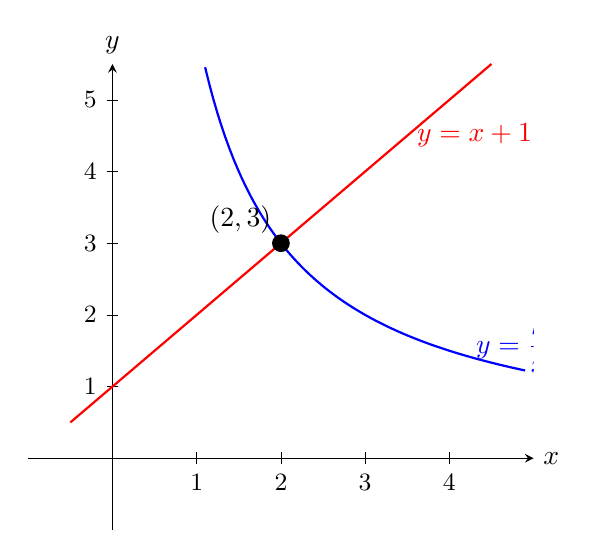
\begin{tikzpicture}
\begin{axis}[
  width=8cm, height=7.5cm,
  axis lines=center,
  xlabel={$x$}, ylabel={$y$},
  every axis x label/.style={at={(axis cs:5.0,0)}, anchor=west},
  every axis y label/.style={at={(axis cs:0,5.5)}, anchor=south},
  xmin=-1.0, xmax=5.0,
  ymin=-1.0, ymax=5.5,
  xtick={1,2,3,4},
  ytick={1,2,3,4,5},
  tick style={color=black},
  ticklabel style={font=\small},
  clip=true,
]
  % y = 6/x (第一象限)
  \addplot[blue, thick, domain=1.1:4.9, samples=80] {6/x};
  \node[right, blue] at (axis cs:4.2, 1.6) {$y=\dfrac{k}{x}$};

  % y = x + 1 (辅助一次函数)
  \addplot[red, thick, domain=-0.5:4.5, samples=20] {x+1};
  \node[right, red] at (axis cs:3.5, 4.5) {$y=x+1$};

  % 交点：6/x = x+1 => x^2+x-6=0 => x=2, y=3
  \addplot[only marks, mark=*, mark size=3pt] coordinates {(2,3)};
  \node[above left] at (axis cs:2,3) {$(2,3)$};
\end{axis}
\end{tikzpicture}
\end{document}
